% Add \usepackage{graphicx} to the preamble.
% Extract the ZIP into the Overleaf project; the PDF is fully vector.
\begin{figure*}[t]
  \centering
  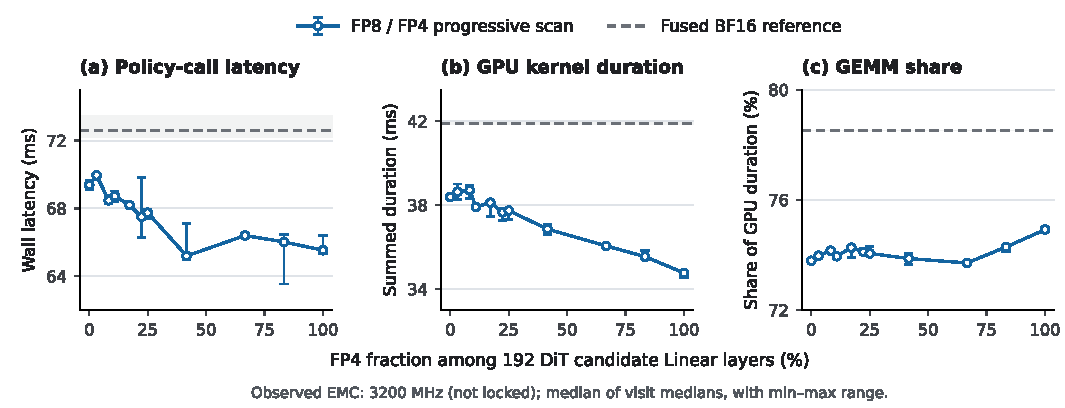
\includegraphics[width=\textwidth]{thor_progressive_performance.pdf}
  \caption{Progressive FP8-to-FP4 quantization on Thor. The 11 measured tiers replace 0, 6, 16, 21, 33, 43, 48, 80, 128, 160, and 192 of the 192 DiT candidate Linear layers with FP4; remaining candidate layers use FP8, and other model layers remain BF16. The dashed line denotes the fused, unquantized BF16 reference. (a) Single complete-policy-call wall latency, excluding between-call reset and logging. (b) Sum of profiled GPU kernel durations. (c) GEMM-family duration, including BMM and GEMV, as a percentage of (b). Only samples assigned to the observed 3200\,MHz EMC stratum are shown; clocks were monitored without locking. Markers are medians of per-visit medians; bars (and the BF16 band) span their minimum and maximum, not confidence intervals. Wall latency and GPU duration were measured separately. These performance results do not establish task-quality equivalence.}
  \label{fig:thor-progressive-performance}
\end{figure*}
